\documentclass[conference]{IEEEtran}
\IEEEoverridecommandlockouts
% The preceding line is only needed to identify funding in the first footnote. If that is unneeded, please comment it out.
%Template version as of 6/27/2024

\usepackage{cite}
\usepackage{amsmath,amssymb,amsfonts}
\usepackage{algorithmic}
\usepackage{graphicx}
\usepackage{textcomp}
\usepackage{xcolor}
\def\BibTeX{{\rm B\kern-.05em{\sc i\kern-.025em b}\kern-.08em
    T\kern-.1667em\lower.7ex\hbox{E}\kern-.125emX}}
\begin{document}

\title{Deep Reinforcement Learning for Adaptive Non-Primary Channel Access in IEEE 802.11bn}
% Remove funding footnote for now - add back if needed
% \thanks{Identify applicable funding agency here. If none, delete this.}

\author{
\IEEEauthorblockN{Taewon Song}
\IEEEauthorblockA{\textit{Dept. of Internet of Things} \\
\textit{Soonchunhyang University}\\
Asan, Republic of Korea \\
twsong@sch.ac.kr}
}

\maketitle

\begin{abstract}
Efficient spectrum utilization is critical in modern Wi-Fi networks as traditional systems require primary channel occupancy for transmission, limiting efficiency in overlapping BSS (OBSS) environments. IEEE 802.11bn introduces non-primary channel access (NPCA) capability, yet optimal decision strategies remain challenging. This paper presents a deep reinforcement learning approach for adaptive NPCA decision-making using Semi-Markov Decision Process formulation with Deep Q-Network. Simulations across varying network scenarios demonstrate significant throughput improvements over baseline strategies, with contention window index as the most critical decision factor. The learning algorithm exhibits conservative strategies favoring long-term stability, providing insights for next-generation Wi-Fi channel access mechanisms.
\end{abstract}

\begin{IEEEkeywords}
Deep Reinforcement Learning, Non-Primary Channel Access, Wi-Fi Networks, Semi-MDP, OBSS, Channel Access, DQN
\end{IEEEkeywords}

\section{Introduction}

Modern wireless networks face increasing challenges in spectrum efficiency as Wi-Fi deployments become denser and user demands grow. Traditional channel access mechanisms, while effective in simple scenarios, struggle to adapt to dynamic interference patterns and varying network conditions.

IEEE 802.11 systems traditionally require the primary channel to be idle before wide-band transmissions can occur \cite{wei2024non}. This constraint leads to significant spectrum waste when secondary channels remain unused despite primary channel occupancy by overlapping BSS (OBSS) traffic. While IEEE 802.11bn introduces non-primary channel access (NPCA) capability \cite{bellalta2025performance}, existing approaches rely on static heuristics that cannot adapt to dynamic network conditions, leaving a critical gap in intelligent decision-making strategies.

Consider a scenario where a station detects OBSS activity on its primary channel while secondary channels are available. The station must decide whether to wait for primary channel access or switch to NPCA, balancing factors such as transmission duration, channel switching overhead, and future network conditions. Such decisions require adaptive intelligence beyond static rules.

In this paper, we describe an intelligent NPCA decision-making framework that enables stations to learn optimal channel access policies through interaction with dynamic network environments. We formulate this as an online learning problem where stations adapt their behavior based on observed network states and reward feedback.

Our approach employs deep reinforcement learning, specifically a Semi-Markov Decision Process (Semi-MDP) formulation with Deep Q-Network (DQN) \cite{mnih2015human}, to capture temporal dependencies in NPCA decisions. The framework enables stations to learn from experience and adapt to varying OBSS patterns and network densities.

The main contributions of this work are:
\begin{itemize}
\item A Semi-MDP framework for NPCA decision-making that captures temporal dynamics and network state transitions
\item A DQN-based learning algorithm that enables adaptive channel access policies in dynamic environments  
\item Comprehensive performance evaluation demonstrating throughput improvements over baseline strategies
\item Analysis of key decision factors revealing the critical role of contention window index in NPCA decisions
\end{itemize}

The remainder of this paper is organized as follows. Section II reviews related work in NPCA and reinforcement learning applications. Section III presents our system model and problem formulation. Section IV describes the proposed DRL framework. Section V presents simulation results and analysis. Finally, Section VI concludes the paper and discusses future work.

\section{Related Work}

NPCA mechanisms have been extensively studied in the context of spectrum efficiency improvement. Traditional approaches rely on heuristic rules and static thresholds for channel switching decisions \cite{wei2024optimized}. However, these methods fail to adapt to dynamic network conditions and varying traffic patterns.

Reinforcement learning has shown promising results in wireless network optimization \cite{mnih2013playing}. Recent works have applied DRL to various wireless problems, including resource allocation and interference management. Semi-MDP formulations have been particularly effective in capturing temporal dependencies in wireless environments \cite{sutton2018reinforcement}.

Existing NPCA studies focus primarily on theoretical analysis and static optimization. This work addresses the gap by proposing an adaptive learning approach that can respond to real-time network dynamics.

\section{System Model and Problem Formulation}

\subsection{NPCA System Model}

We consider a wireless network with overlapping BSSs where stations operate on a primary channel (Channel 0) and can access a secondary NPCA channel (Channel 1) when OBSS activity is detected. Each station maintains awareness of primary channel occupancy and makes binary decisions: stay on primary (Action 0) or switch to NPCA (Action 1).

\subsection{Semi-MDP Formulation}

We formulate the NPCA decision problem as a Semi-MDP with the following components:

\textbf{State Space}: The state $s_t$ includes:
\begin{itemize}
\item Primary channel OBSS occupation time
\item Radio transition time
\item Transmission duration
\item Contention window index
\end{itemize}

\textbf{Action Space}: Binary actions $a_t \in \{0, 1\}$ where 0 represents staying on primary channel and 1 represents switching to NPCA channel.

\textbf{Reward Function}: Rewards are based on successful PPDU transmission length, with zero reward for transmission failures.

The state transition probability follows:
\begin{equation}
P(s_{t+1}|s_t, a_t) = \mathbb{P}[\text{next state} | \text{current state, action}]\label{eq:transition}
\end{equation}

The Q-function update in our DQN framework is:
\begin{equation}
Q(s_t, a_t) \leftarrow Q(s_t, a_t) + \alpha[r_t + \gamma \max_{a'} Q(s_{t+1}, a') - Q(s_t, a_t)]\label{eq:qupdate}
\end{equation}

\section{Proposed DRL Framework}

\subsection{Semi-MDP Learner Architecture}

Our \texttt{SemiMDPLearner} class implements a DQN-based learning algorithm with experience replay and target network stabilization. The neural network architecture consists of fully connected layers with ReLU activations, mapping state observations to Q-values for each action.

\subsection{Training Process}

The learning process follows these key steps:
\begin{enumerate}
\item State observation and action selection using $\epsilon$-greedy policy
\item Experience storage in replay memory buffer
\item Batch sampling and Q-network updates
\item Target network periodic synchronization
\item Exploration rate decay over episodes
\end{enumerate}

\subsection{Network Architecture and Hyperparameters}

The DQN consists of three hidden layers (128, 128, 64 neurons) with dropout regularization. Key hyperparameters include learning rate $\alpha = 0.001$, discount factor $\gamma = 0.99$, and replay memory capacity of 10,000 transitions.

\section{Simulation Results}

\subsection{Experimental Setup}

Simulations are conducted using a time-slotted framework with slot duration of 9 $\mu$s following IEEE 802.11ax standards. We evaluate networks with varying numbers of stations per channel, comparing DRL-based NPCA against baseline approaches including offload-only and local-only strategies.

\subsection{Performance Metrics}

We measure:
\begin{itemize}
\item Throughput: Successful data transmission rate
\item Channel utilization: Ratio of successful channel occupation
\item Fairness: Inter-BSS performance balance
\item Learning convergence: Episode reward progression
\end{itemize}

\subsection{Performance Comparison}

Results demonstrate that the DRL-based approach achieves superior performance compared to static strategies. Across different network scenarios, our method shows significant throughput improvement over baseline approaches including offload-only and local-only strategies. The learning algorithm effectively adapts to varying OBSS patterns and channel conditions.

\subsection{Decision Factor Analysis}

Analysis reveals that contention window index serves as the most critical decision factor, followed by OBSS occupation time. The learned policy exhibits conservative behavior, favoring long-term stability over aggressive short-term gains.

\section{Conclusion and Future Work}

This paper presented a DRL-based approach for adaptive NPCA decision-making in IEEE 802.11bn networks. The Semi-MDP formulation with DQN learning enables stations to intelligently choose between primary and secondary channel access based on dynamic network conditions.

Key findings include the importance of contention window index as a decision factor and the effectiveness of conservative learning strategies. Future work will explore multi-agent learning scenarios and adaptive frame duration optimization based on real-time network conditions.

\begin{table}[htbp]
\caption{Simulation Parameters}
\begin{center}
\begin{tabular}{|l|l|}
\hline
\textbf{Parameter} & \textbf{Value} \\
\hline
Simulation time & 500,000 $\mu$s \\
Slot duration & 9 $\mu$s \\
Number of channels & 2 $\times$ 20 MHz \\
STAs per channel & 2, 6, or 10 \\
Frame duration (Short) & 33 slots (297 $\mu$s) \\
Frame duration (Long) & 165 slots (1485 $\mu$s) \\
OBSS generation rate & 0.05 per slot \\
NPCA switching delay & 5 slots \\
Learning rate & 0.001 \\
Discount factor & 0.99 \\
\hline
\end{tabular}
\label{tab:params}
\end{center}
\end{table}

\begin{figure}[htbp]
\centerline{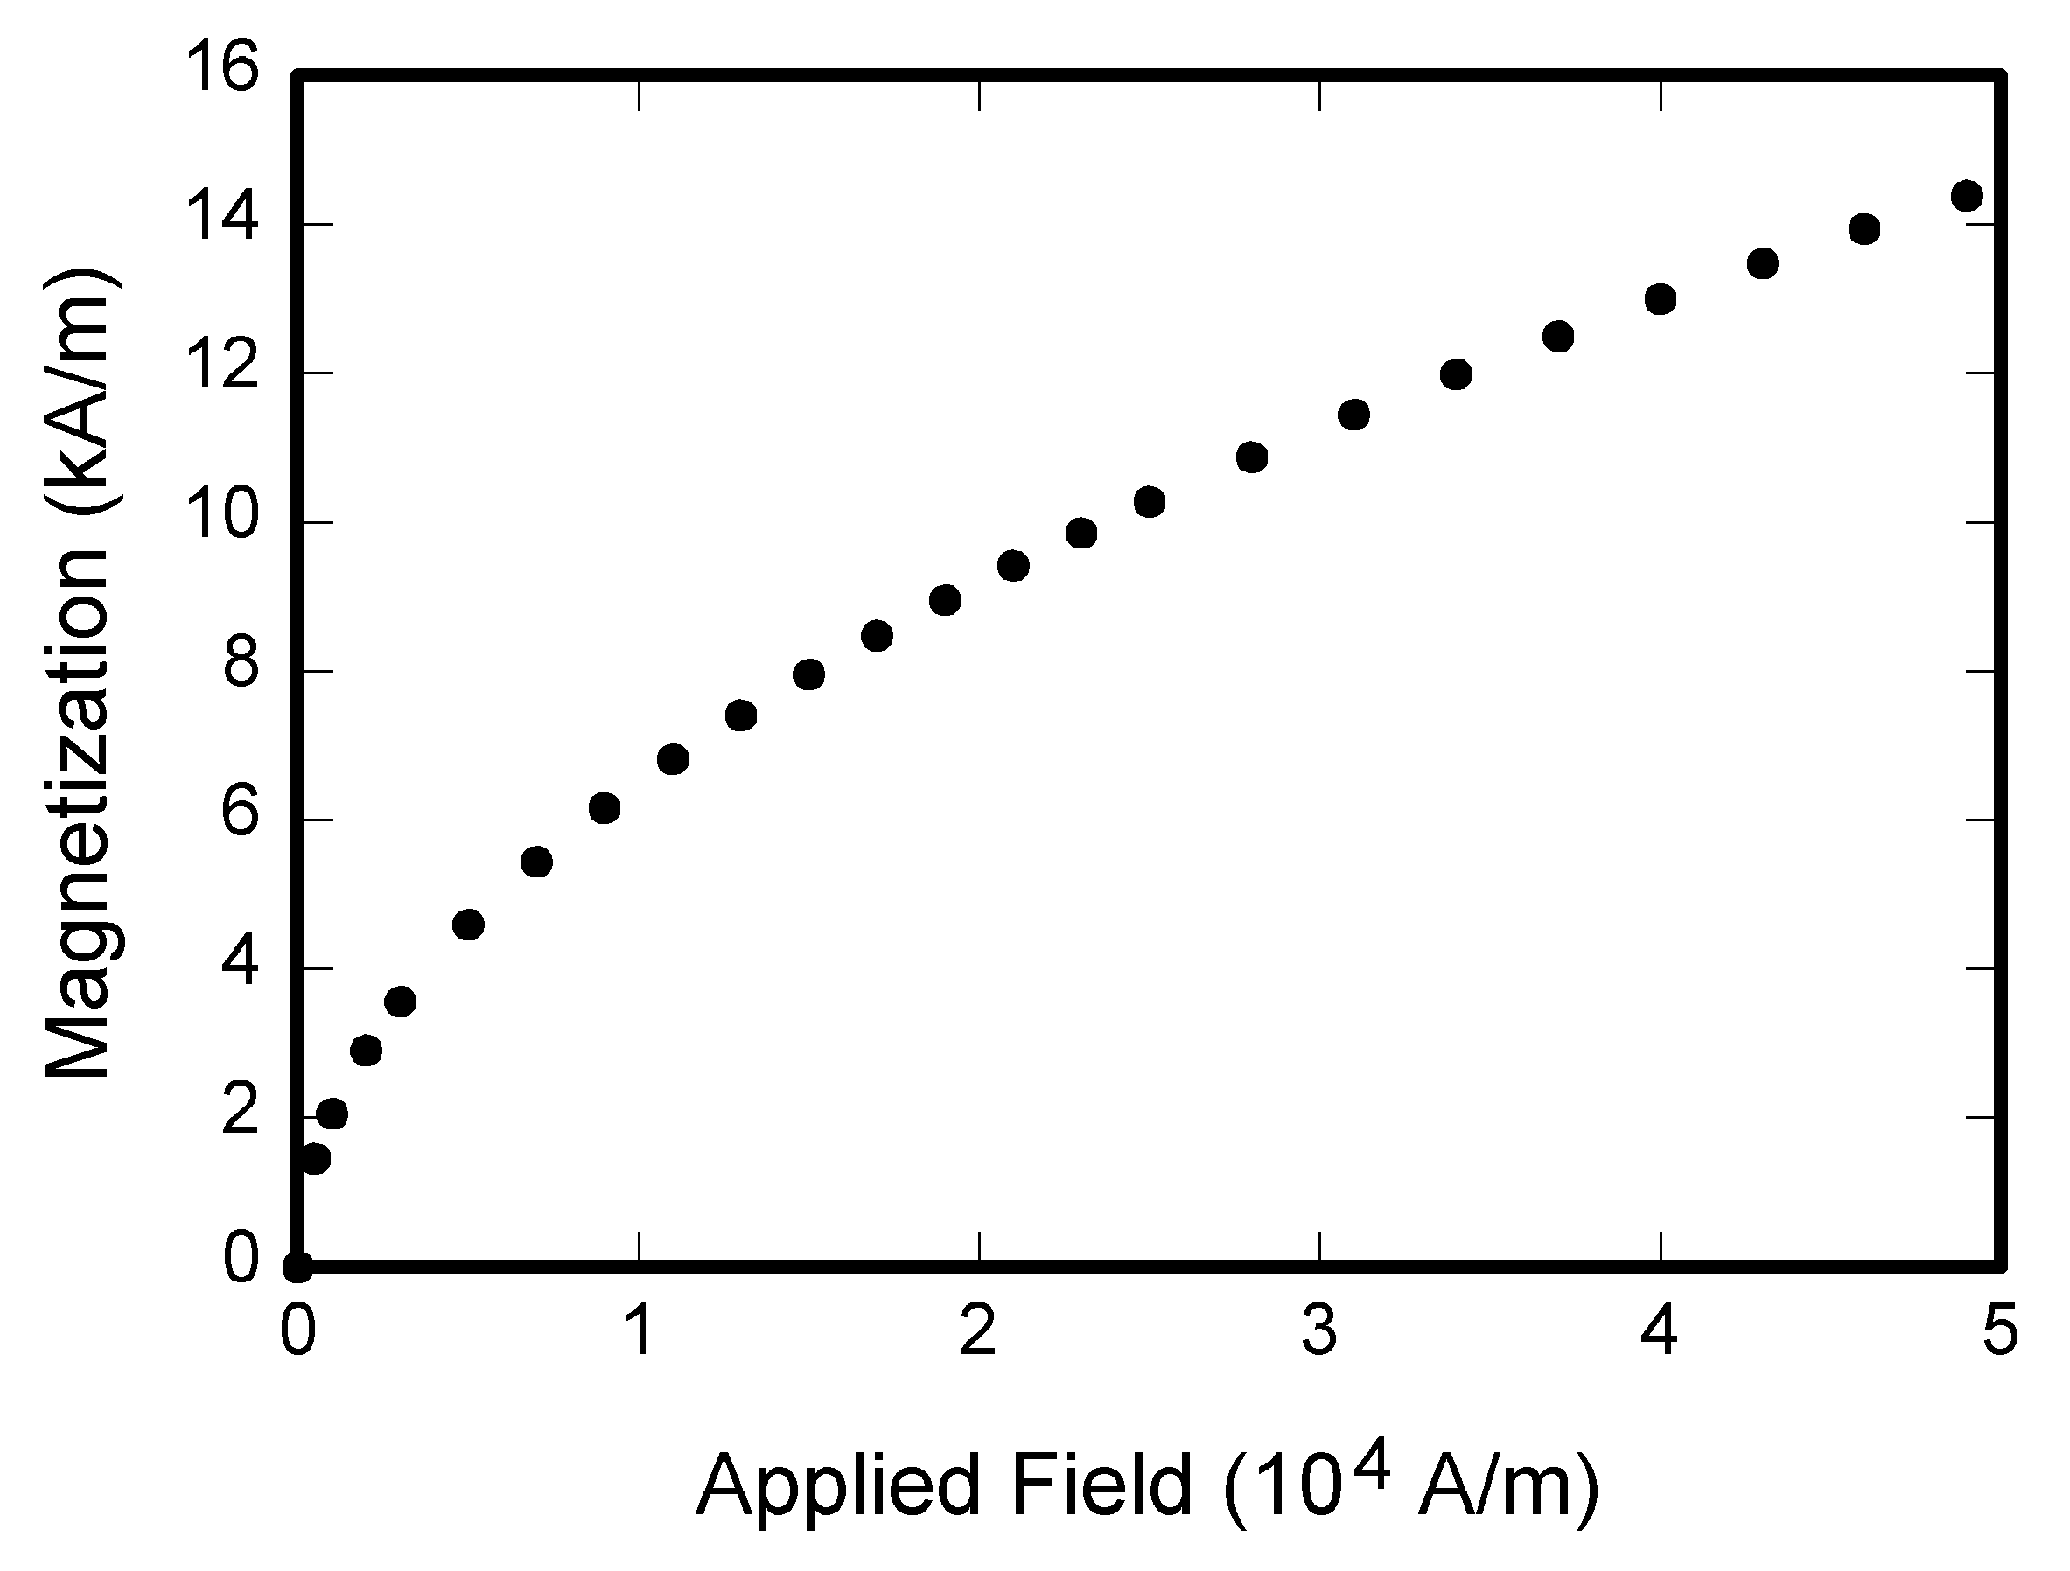
\includegraphics{fig1.png}}
\caption{Training convergence showing episode rewards over time for DRL-based NPCA learning in different network densities.}
\label{fig:training}
\end{figure}

\section*{Acknowledgment}

This research was supported by the MSIT (Ministry of Science and ICT), Korea, under the National Program for Excellence in SW, supervised by the IITP (Institute of Information \& Communications Technology Planning \& Evaluation) in 2025 (2021-0-01399).


\bibliographystyle{IEEEtran}
\bibliography{npca_references}


\end{document}
